\newpage
\part{Introduction}
%\section{Introduction}

\section{Terminologies \& Intros }

\subsection{Categories of Business Analytics}
\begin{itemize}
	\item descriptive analytics
		\begin{itemize}
			\item data engineering(organizing data, queries) \& statistics (mean, trend, standard deviation, test hypotheses)
		\end{itemize}
	
	 \item predictive analytics
	 	\begin{itemize}
	 		\item machine learning \& econometrics
	 		\item learn the pattern of data
	 	\end{itemize}
 	
 	\item prescriptive analytics
 	\begin{itemize}
 		\item algorithm \& optimization models
 	\end{itemize}
	
\end{itemize}

\subsection{From Data to Information}
\begin{figure}[H]
	\centering
	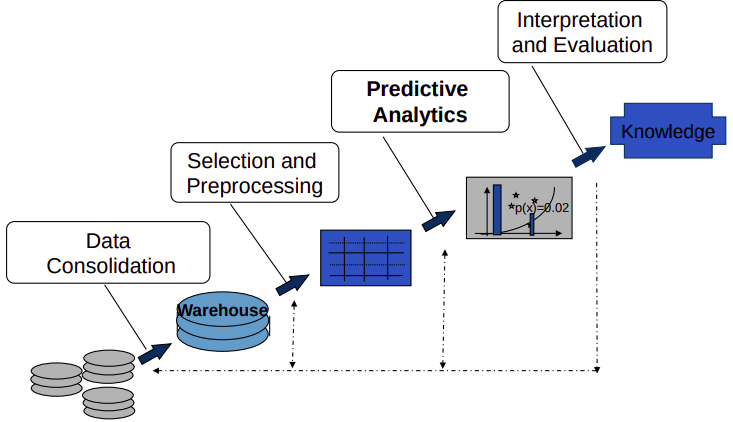
\includegraphics[width=0.8\textwidth]{datatoinfo.png}
\end{figure}

\subsection{Types of Analytic Exercises}
\begin{itemize}
	\item Numeric Prediction
	\begin{itemize}
		\item \textbf{supervised} learning
		\item input: a collection of data input + \textbf{known} output
		
			  job: create a function  $f(\text{input}_{0}) = \text{output}_0$
			  
			  output: \textbf{prediction} values to a \textbf{new} collection of data: $f(\text{input}_1) = ?$ 
		\item example: linear regression
	\end{itemize}

	\item Classification
	\begin{itemize}
		\item \textbf{supervised} learning
		\item input: a collection of data input + \textbf{known} label
			
			  job: create a classifier $f(\text{input}_0) = \text{label}_0$
			  
			  output: \textbf{prediction} label to a \textbf{new} collection of data: $f(\text{input}_1) = ?$
	\end{itemize}

	\item Clustering
	\begin{itemize}
		\item \textbf{unsupervised} learning
		\item input: a collection of data input
			  
			  job: identify "natural" grouping in data
			  
			  output: clustered data
	\end{itemize}

	\item Association Rule Analysis
	\begin{itemize}
		\item \textbf{unsupervised} learning
		\item input: a collection of data list
			  
			  job: identify \textbf{relationships} in data from \textbf{co-occuring items}
		\item grocery store purchases analysis
	\end{itemize}
\end{itemize}

\subsection{Machine Learning Terminology in categorizing analytic exercises}
\begin{itemize}
	\item \textbf{supervised learning}
	\begin{itemize}
		\item a training set is given
		\item find relationship between input \& target attributes		
		\item examples: numeric prediction, classification
	\end{itemize}

	\item \textbf{unsupervised learning}
	\begin{itemize}
		\item only input data available, no training set
		\item find regularities, irregularities, relationships, similarities among data points
		\item examples: clustering, association rule analysis
	\end{itemize}
\end{itemize}

\subsection{Model}
examples: 
\begin{itemize}
	\item linear model
	\item decision tree
	\item neural network
\end{itemize}

\section{Statistics Recap}
\subsection{Categories}
\begin{itemize}
	\item \hl{descriptive statistics}: \textbf{summary} of data
	
	\begin{itemize}
		
		\item examples: mean, standard deviation
	\end{itemize}
	
	\item \hl{inferential statistics}: model \textbf{patterns} of data, accounting for \textbf{randomness} and drawing \textbf{inferences about a larger population}
	\begin{itemize}
		\item estimation
		\item hypothesis testing
		\item forecasting
		\item correlation
		\item regression
	\end{itemize}
	
\end{itemize}

\subsection{Random Variables}
$X$ is a \textbf{random variable} if:
\begin{itemize}
	\item it represents a \textbf{random draw} from a population
	\item it's associated with a \textbf{probability distribution}
	\item either \textbf{discrete} or \textbf{continuous}
	\item example: a random variable that follows a \textbf{normal distribution} $N(\mu, \sigma^2)$ has a probability density function of 
	$$f(x) = \frac{1}{\sigma \sqrt{2\pi}}e^{-\frac{(x-\mu)^2}{2\sigma^2}}$$
\end{itemize}

\subsection{Normal Distribution \& Standard Normal Distribution}
A random variable $X$ follows a normal distribution $N(\mu, \sigma^2)$

To \textbf{''standardize''} a random variable $x$ to \textbf{standard normal distribution }
$N(0,1)$: $$Z = \frac{X - \mu}{\sigma}$$

\subsection{Probability density function \& Cumulative density function}
\textbf{Probability density function (pdf): f(x)} $$f(x) = P(X = x)$$

\textbf{Cumulative distribution fuction (cdf): F(x)} $$F(x) = P(X \leq x)$$ $$P(X \geq x) = 1 - F(x)$$  $$P(x_1 \leq X \leq x_2) = F(x_2) - F(x_1)$$

\subsection{Statistical Estimation}
\textbf{Statistical estimation}: 

The parameters of a population are \textbf{unknown}. However, we can \textbf{estimate} the parameters by \textbf{drawing a random sample} out of the population, analyzing this random sample and getting the statistics. The statistics should infer the parameters.
\\ \ \\
Requirements of random sampling: 
\begin{itemize}
	\item each variable $X$ from the population is a random variable. 
	\item each combination of $n$ sample points has an \textbf{equal} chance of being selected.  
	
\end{itemize}
	$\longrightarrow$ a random sample is a set of \textbf{independent, identically distributed (i.i.d)} random variables.
\\ \ \\
\textbf{Categories:}
\begin{itemize}
	\item Point Estimate
	\begin{itemize}
		\item sample mean
		\item sample proportion
	\end{itemize}

	\item Interval Estimate
	\begin{itemize}
		\item \textbf{confidence interval} for sample mean
		\item \textbf{confidence interval} for sample proportion
	\end{itemize}
\end{itemize}
Point estimate is always within the interval estimate.

\subsubsection{Point Estimate: Population Mean and Its Estimation}
\begin{itemize}
	\item \textbf{Expected Value of X and the Population Mean}
	
	The expected value of a probability \textbf{weighted average} of $X$, $E(X)$, is the mean/expected value of the probability distribution of $X$. 
	
	$f(x_i)$ is the (discrete) probability that $X = x_i$.
	$$\mu_x = E(X) = \Sigma_{i=1}^{n} x_i f(x_i)$$ or $$\mu_x = E(X) = \int_{-\infty}^{+\infty} xf(x) dx$$ 
	
	If this random sample is a set of i.i.d random variables, the \textbf{expected value of X} is the \textbf{population mean}(unknown).
	
	\item \textbf{Estimation of the Population Mean by Sample Mean}
	
	\textbf{Sample Mean $\bar{X}$:} the \textbf{random variable} for the arithmetic mean of the sample. $\bar{x}$ is the mean of a \textbf{particular realization} of a sample.
	
	 
	$$\bar{X} = \frac{\Sigma X_i}{n} $$
	
	This is a random variable, because a lot of samples are drawn repeatedly, the arithmetic mean of the sample has also a probability distribution. \textbf{The mean(center) of this distribution should estimate the mean of the whole population. }
	
	
	
	\item Requirements for an estimator: \textbf{unbiased}
	
	Example: $$E(\bar{X}) = \mu_x$$
	
	\item \textbf{Standard Error of the Sample Mean}: 
	
	\begin{itemize}
		\item  \hl{\textbf{standard error of the sample mean $SE_{\bar{X}}$}} : an estimate of how far the \textbf{sample mean} is likely to be \textbf{from the population mean}. 
		
		When $n \rightarrow \infty$,  $SE_{\bar{X}}  \rightarrow \sigma_{\bar{X}}$ (\hl{\textbf{true standard deviation of sample mean}}).
		
		$$SE_{\bar{X}} = \frac{s}{\sqrt{n}}$$
		$$\sigma_{\bar{X}} = SD(\bar{X}) = \sqrt{Var(\bar{X})} = \frac{\sigma}{\sqrt{n}}$$
		
		\item\hl{\textbf{sample standard deviation $s$}} : the degree to which \textbf{individuals within the sample} differ from the \textbf{sample mean}
		
		$$s = \sqrt{\frac{1}{n-1} \Sigma_{i=1}^{n} (X_i - \bar{X})^2}$$
	\end{itemize}
	
	\item \textbf{Law of Large Numbers}
	
	If $n \rightarrow \infty, \bar{X}_n \rightarrow \mu$. 
	
	If the size of the random sample is large enough, then the arithmetic mean converge to the real population mean.  
	$$\lim\limits_{n\rightarrow \infty} P(|\bar{X}_n - \mu| > \epsilon) = 0$$
	
	\item \textbf{Central Limit Theorem}
	
	If \textbf{$n \rightarrow \infty$}, the \textbf{average $\bar{X}$} of any population of \textbf{i.i.d.} random variables $X_i$ with the population mean $\mu_X$ and population variance $\sigma^2$ \textbf{follows asymptotically a normal distribution} $\bar{X} \sim N(\mu_X, \frac{\sigma^2}{n})$. 
	$$\bar{X} = \frac{X_1 + X_2 + \dots + X_n}{n}$$
	The \textbf{standardize average} $Z \sim N(0,1)$: $$Z = \frac{\bar{X} - \mu_X}{\frac{\sigma}{\sqrt{n}}}$$
\end{itemize}

\subsubsection{Interval Estimate: }
\begin{itemize}
	\item \textbf{Confidence Interval of Sample Mean:}
	\begin{itemize}
		\item Assumption: samples drawn from a population that follows a normal distribution $N(\mu_X, \sigma^2)$. 
		
		eg: The sample mean $\bar{X}$ follows asymptotically a normal distribution $N(\mu_X, \frac{\sigma^2}{n})$
		\item a level of confidence($1 - \alpha$) is given.
		\item \textbf{two-sided} $\rightarrow z_{(1 - \frac{\alpha}{2})} $  / $z_{(1 + \frac{\alpha}{2})}$
		\item z value: \textbf{standardized}. \textbf{Find z value from cdf-table given an $\alpha$}.
		\item if population standard deviation $\sigma$ is given, 
		$$CI = \left[ \bar{X} - z_{(1 - \frac{\alpha}{2})}\cdot \frac{\sigma}{\sqrt{n}} , \bar{X} + z_{(1 - \frac{\alpha}{2})}\cdot \frac{\sigma}{\sqrt{n}} \right] $$
		$$Pr(\bar{X} - z_{(1 - \frac{\alpha}{2})}\cdot \frac{\sigma}{\sqrt{n}} < \mu_X < \bar{X} + z_{(1 - \frac{\alpha}{2})}\cdot \frac{\sigma}{\sqrt{n}} ) = 1 - \alpha$$
		
		\item if population standard deviation $\sigma$ is unknown, 
		\begin{itemize}
			\item n is \textbf{small}: use \textbf{sample standard deviation $s$} and \textbf{t-distribution}
			$$CI = \left[ \bar{X} - t_{(1 - \frac{\alpha}{2})}\cdot \frac{s}{\sqrt{n}} , \bar{X} + t_{(1 - \frac{\alpha}{2})}\cdot \frac{s}{\sqrt{n}} \right] $$
			\item n is \textbf{large}: use \textbf{sample standard deviation $s$} and \textbf{normal distribution}
			$$CI = \left[ \bar{X} - z_{(1 - \frac{\alpha}{2})}\cdot \frac{s}{\sqrt{n}} , \bar{X} + z_{(1 - \frac{\alpha}{2})}\cdot \frac{s}{\sqrt{n}} \right] $$
		\end{itemize}
		If $n \rightarrow \infty$, the T-Distribution converges to a Normal Distribution.
		
	\end{itemize}

	\item Effects on Confidence Intervals:
	\begin{itemize}
		\item \textbf{sample size} n: n $\uparrow$, interval size $\downarrow$ 
		
		(the larger the size, more precise is the estimation)
		\item \textbf{confidence level} ($1 - \alpha$): confidence level $\uparrow$, interval size $\uparrow$ 
		
		(given the same sample size, the higher the confidence level, the more values need to be included.)
		\item \textbf{population standard deviation} $\sigma$: $\sigma \uparrow$, interval size $\uparrow$ 
		
		(the more spreaded the population, the more values need to be included to achieve same confidence level.)
	\end{itemize}
\end{itemize}

\subsection{Statistical Tests}
\subsubsection{Process} 
\begin{itemize}
	\item number of samples
	\begin{itemize}
		\item 1 sample:
		\begin{itemize}
			\item $\sigma$ known: \textbf{Z-Test}
			\item $\sigma$ unknown: \textbf{T-Test}
		\end{itemize}
		\item 2 samples:
		\begin{itemize}
			\item dependent:\textbf{ Paired T-Test} 
			\item independent: \textbf{Welch-Test}
		\end{itemize}
	\end{itemize}
	\item Formulate \textbf{null and alternative hypothesis} ($H_0$ and $H_1$), $H_1$ is the hypothesis we want to test.
	\item Choose an \textbf{$\alpha$ level}. (type I error: probability of falsely rejecting $H_0$)
	\item Find corresponding \textbf{distribution}, calculate \textbf{test statistic}, 
	\item Find the \textbf{critical value} in the table and corresponding \textbf{p-value}
	\item Conclusion: 
	\begin{itemize}
		\item $p \leq \alpha$, reject $H_0$
		\item $p > \alpha$, reject $H_1$ 
	\end{itemize}
	Interpretation of p-value: the probability of having the other mean $\bar{x}$, given that $H_0$ is true.
\end{itemize}

\subsubsection{Two-sided or One-sided Test}
Three possible alternative hypotheses $H_1$:
\begin{figure}[H]
	\centering
	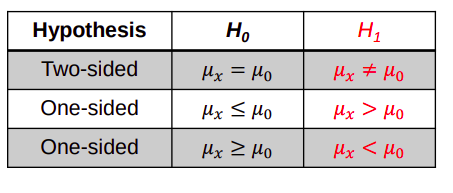
\includegraphics[width=0.5\textwidth]{H1.png}
\end{figure}
Critical Value:
\begin{itemize}
	\item two-sided test: $z_{\frac{\alpha}{2}}, z_{1-\frac{\alpha}{2}}$ / $t_{\frac{\alpha}{2}}, t_{1-\frac{\alpha}{2}}$
	\item one-sided test: $z_{1-\alpha}$ / $t_{1-\alpha}$
\end{itemize}



\subsubsection{Z-Test}
\begin{itemize}
	\item Requirements: \textbf{1 sample, $\mu$, $\sigma$ known} (population mean and population standard deviation)  
	\item Distribution: \textbf{standardized normal distribution}
	\item test statistic: \large{$$ z = \frac{\bar{X} - \mu_0}{\frac{\sigma}{\sqrt{n}}}$$}
	\item critical value: $z^c_{1-\frac{\alpha}{2}}$ / $z^c_{1-\alpha}$
	\item $H_0$ Rejection region/ $H_1$ Acceptance region :
	
	\begin{table}[H]
		\begin{center}
			\begin{tabular}{|c|c|c|}
				\hline
				$H_1$ 				& Rejection Region					& test variant \\ \hline
				$\mu\mu \neq \mu_0$	& $|z| \geq z^c_{1-\frac{\alpha}{2}}$	& two-sided                 \\ \hline
				$\mu\mu > \mu_0$	& $ z \geq z^c_{1-\alpha}$			& one-sided                  \\ \hline
				$\mu\mu < \mu_0$	& $ z \leq -z^c_{1-\alpha} $			& one-sided                  \\ \hline
			\end{tabular}
		\end{center}
	\end{table} 	
\end{itemize}

\subsubsection{Single Sample T-test}
\begin{itemize}
	\item Requirements: \textbf{1 sample, $\sigma$ unknown}
	\item Distribution: Student \textbf{t-Distribution}
	\item Degree of Freedom($df$): determines how spread the distribution is. 
	\large{$$df = n - 1$$}
	\item test statistic: 
	
	$s$ is the standard error(empirical)
	\large{$$t(df) = \frac{\bar{X} - \mu_0}{\frac{s}{\sqrt{n}}}$$}
	\item critical value: $t^c_{1-\frac{\alpha}{2}, df}$ / $t^c_{1-\alpha, df}$
	\item $H_0$ Rejection region/ $H_1$ Acceptance region :
	
	\begin{table}[H]
		\begin{center}
			\begin{tabular}{|c|c|c|}
				\hline
				$H_1$ 				& Rejection Region					& test variant \\ \hline
				$\mu\mu \neq \mu_0$	& $|t| \geq t^c_{1-\frac{\alpha}{2}, df}$	& two-sided                 \\ \hline
				$\mu\mu > \mu_0$	& $ t \geq t^c_{1-\alpha, df}$			& one-sided                  \\ \hline
				$\mu\mu < \mu_0$	& $ t \leq -t^c_{1-\alpha,df} $			& one-sided                  \\ \hline
			\end{tabular}
		\end{center}
	\end{table} 		
\end{itemize}

\subsubsection{Paired Sample T-test}
\begin{itemize}
	\item Requirements: \textbf{2 samples, $\sigma$ unknown, dependent}
	
	eg: means obtained in 2 conditions(time,places,etc.) by a single group of participants
	\item Distribution: \textbf{T-Distribution}
	\item Test of relationship between 2 linked samples (eg: Difference)
	\item Degree of Freedom($df$): $$df = n -1 $$
	\item Example null hypothesis: $ H_0: \mu_d = \mu_1 - \mu_2 = \Delta_0$
	\item test statistic: 
	\large{$$t = \frac{\bar{d} - \Delta_0}{\frac{s}{\sqrt{n}}}$$}
	\item critical value: $t^c_{1-\frac{\alpha}{2}, df}$ / $t^c_{1-\alpha, df}$
	\item $H_0$ Rejection Region/ $H_1$ Acceptance Region:
	\begin{table}[H]
		\begin{center}
			\begin{tabular}{|c|c|c|}
				\hline
				$H_1$ 				& Rejection Region					& test variant \\ \hline
				$\mu_d \neq \Delta_0$	& $|t| \geq t^c_{1-\frac{\alpha}{2}, df}$	& two-sided                 \\ \hline
				$\mu_d > \Delta_0$	& $ t \geq t^c_{1-\alpha, df}$			& one-sided                  \\ \hline
				$\mu_d < \Delta_0$	& $ t \leq -t^c_{1-\alpha,df} $			& one-sided                  \\ \hline
			\end{tabular}
		\end{center}
	\end{table} 	
\end{itemize}

\subsubsection{Independent T-Test/ Welch-Test}
\begin{itemize}
	\item Requirements: \textbf{2 samples, $\sigma$ unknown, independent}
	
	eg: credit card debt difference between urban and rural households/ shopping expenses between male and female
	\item Distribution: \textbf{T-Distribution}
	\item Test of relationship between 2 independent samples (doesn't need to be same size)
	\item Degree of Freedom($df$): round to \textbf{nearest integer} number
	\large{$$df = \dfrac{(\frac{s_1^2}{n_1} + \frac{s_2^2}{n_2})^2}{\frac{(\frac{s_1^2}{n_1})^2}{n_1 -1} + \frac{(\frac{s_2^2}{n_2})^2}{n_2 -1}}$$} 
	\item test statistic:
	\large{$$t = \frac{(\bar{x}_1 - \bar{x}_2) - \mu_0}{s_{\bar{x}_1 -\bar{x}_2}}$$}
	\large{$$s_{\bar{x}_1 -\bar{x}_2} = \sqrt{\frac{s_1^2}{n_1} + \frac{s_2^2}{n_2}}$$}
	\item $H_0$ Rejection Region/ $H_1$ Acceptance Region:
	\begin{table}[H]
		\begin{center}
			\begin{tabular}{|c|c|c|}
				\hline
				$H_1$ 				& Rejection Region					& test variant \\ \hline
				$\mu_d \neq \Delta_0$	& $|t| \geq t^c_{1-\frac{\alpha}{2}, df}$	& two-sided                 \\ \hline
				$\mu_d > \Delta_0$	& $ t \geq t^c_{1-\alpha, df}$			& one-sided                  \\ \hline
				$\mu_d < \Delta_0$	& $ t \leq -t^c_{1-\alpha,df} $			& one-sided                  \\ \hline
			\end{tabular}
		\end{center}
	\end{table} 
	\item Confidence Interval of both samples: if both confidence intervals overlap each other $\rightarrow$ \textbf{cannot reject} $H_0$
\end{itemize}
\subsubsection{Using Confidence Intervals in Significance Tests}
Find confidence intervals for $\mu_x$, which -- under $H_0$ -- contains the true value $\mu_x$ with a probability of at least $1 - \alpha$: 
\begin{itemize}
	\item $\sigma$ known: \textbf{Normal Distribution}
	$$CI = [\bar{x} - z^c_{(1-\frac{\alpha}{2})} \cdot \frac{\sigma}{\sqrt{n}}, \bar{x} + z^c_{(1-\frac{\alpha}{2})} \cdot \frac{\sigma}{\sqrt{n}}]$$
	\item $\sigma$ unknown: \textbf{t-Distribution}
	$$CI = [\bar{x} - t^c_{(1-\frac{\alpha}{2}, n-1)} \cdot \frac{s}{\sqrt{n}}, \bar{x} + t^c_{(1-\frac{\alpha}{2}, n-1)} \cdot \frac{s}{\sqrt{n}}]$$
\end{itemize}	
Conclusion:
\begin{itemize}
	\item Accept $H_0$: if $\mu_0$ lies \textbf{within} the confidence interval
	\item Rejection $H_0$: if $\mu_0$ lies \textbf{outside} the confidence interval
\end{itemize}

\subsubsection{Other Tests}
\begin{itemize}
	\item Parametric Tests: eg: T-tests,  F-test(comparing variance of 2 samples)
	\item Non-parametric Tests: eg: Wilcoxon signed-rank test(2 paired i.i.d. samples), Mann-Whitney-U test(2 independent i.i.d. samples)
	\item Test of Probability Distribution: Kolmogorov-Smirnov test, Chi-square test
\end{itemize}

\section{Description of a Dataset}
\begin{itemize}
	\item \textbf{Dependent} and \textbf{independent} variables
	\item Scales of measurement of the variables 
	\begin{figure}[H]
		\centering
		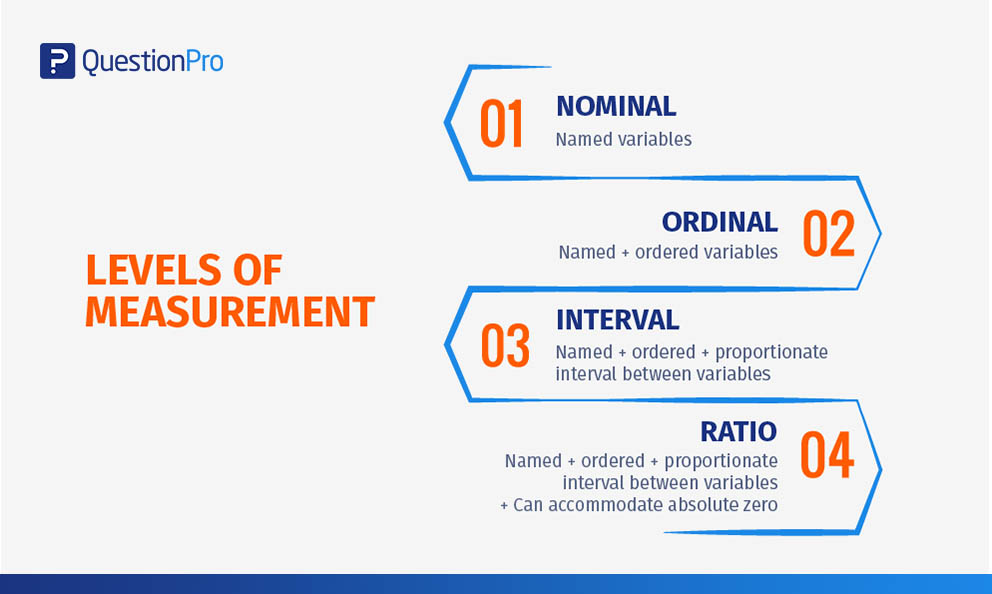
\includegraphics[width=0.8\textwidth]{scale_measurement.jpg}
	\end{figure}
	\begin{itemize}
		\item \textbf{Nominal}: \textbf{categorical} variable scale. A scale used for labeling variables into distinct classifications, \textbf{doesn't involve quantitative value or order. }
		\begin{itemize}
			\item eg: Gender, City, Nationality, Jobs
		\end{itemize}
		\item \textbf{Ordinal}: scale to depict \textbf{order} of the variables for non-mathematical ideas. It maintains a \textbf{descriptional} quality and the \textbf{difference between variables can't be calculated}. 
		\begin{itemize}
			\item eg: Frequency(high, medium, low), Happiness, Satisfaction, Pain level, Cloth size (S, M, L), rank of Unis
		\end{itemize}
		\item \textbf{Interval}: numeric scale where \textbf{order} of the variables as well as the \textbf{difference between variables are known}. There exists \textbf{no true 0}. Variables can be added and subtracted, but \textbf{not multiplied or divided}. 
		\begin{itemize}
			\item eg: GPA, GRE, Celsius, Fahrenheit (20$^\circ$C is 10$^\circ$C higher than 10$^\circ$C, it doesn't mean 2 times warmer.)
		\end{itemize}
		\item \textbf{Ratio}: numeric scale that's ordered, difference between variables known, and there \textbf{exists true 0}. Variables can be added, subtracted, multiplied and divided.
		\begin{itemize}
			\item eg: weight, height, time, Kelvin temperature, money
		\end{itemize}
	\end{itemize}
	\item \textbf{Cross-sectional, time series, panel data} (see 7.1.5)
\end{itemize}


%\section{Summary of Possible Exam Questions}
%\begin{itemize}
%	\item Calculation of arithmetic weighted mean of sample $\bar{X}$, variance $\sigma^2$ of the sample, standard deviation $\sigma$ of the sample.
%	\item Calculation of variance/standard deviation of the sample mean $\sigma_{\bar{X}}^2$/$\sigma_{\bar{X}}$
%	\item Standardization of a normal distribution 
%	\item Calculation of probability, find values from pdf or cdf table 
%	\item independent, identically distributed sample points (i.i.d.)
%	\item Performance of Significance Test according to requirements
%	\item p-value: Interpretation when to reject $H_0$ ($p < \alpha$)
%	\item description of dataset
%\end{itemize}
